\section{Experimental results}\label{sec:experiments}

\noindent\textbf{Proof-of-work}

\noindent
We have experimentally analyzed the egalitarianism of proof-of-work coins
Bitcoin, Litecoin, Ethereum, and Monero. We chose these four as a representative
sample among the thousands of existing cryptocurrencies. Bitcoin represents the
largest and most successful cryptocurrency by market cap. Litecoin is the first
cryptocurrency which aimed to become more egalitarian by replacing Bitcoin's
SHA256 work function with scrypt, a more memory-hard function. Ethereum is one
of the most promising cryptocurrencies, the first to support smart contracts,
and second largest by market cap; their work function is different from both
Bitcoin and Litecoin. Finally, Monero is a special case, because it claims
strong egalitarianism due to its memory-hard mining function, Cryptonight.
Furthermore, its protocol is often updated to maintain egalitarianism.

As expected, we show that Bitcoin is the least egalitarian of the four. Ethereum
follows next. Litecoin is more egalitarian, due to its use of scrypt. Finally,
Monero is the most egalitarian among the proof-of-work coins we have studied.

\dionyziz{Revise above results based on experimental data.}

For our experimental setting, we worked as follows. First, we collected empirical
data which describe the available mining hardware options in the market. For
each machine choice, we determined the cost of investment. This is comprised
of its initial price to purchase (in USD) as well as its energy cost of
operation (in watts). The cost of operation was translated to USD per hour by
considering the electricity cost of KWh. As a reference, we used the KWh cost in
the United States in which $1$ KWh costs $0.10\$$. We remark that this reference
electricity cost is only for estimation and can vary depending on the country of
operation, contractual miner agreements with the power grid, or bulk pricing.
While we do extract exact numbers using this as our experimental basis, we note
here that the qualitative difference of egalitarianism across cryptocurrencies
(i.e., the shape of their egalitarian curve and the order of egalitarianism of
different cryptocurrencies) remains the same if the electricity cost is
adjusted.

\dionyziz{modify the above electricity cost to correspond to the data we use.}

\dionyziz{confirm that this adjustment maintains curve shapes?}

We then use the reported hash rate of the machine to extract an expectation of
the freshly mined coins it would generate per unit of time, if it were to run
continuously. This expectation is taken over the randomness of all honest
blockchain protocol executions. As such, each party is awarded block rewards in
proportion to their computational power. The difference between revenue per unit
of time and cost of operation per unit of time produces an \emph{income rate}
which is measured in USD per hour.

For our experiments, we use a duration of investment of $d = 1$
year. This choice of parameter is made arbitrarily to correspond to the usual
definition of ROI in traditional finance. Again this parameter does not make a
qualitative difference in our metrics.

\dionyziz{confirm that this adjustment maintains curve shapes?}

To find the optimal investment strategy, we employ the following algorithm. The
initial capital available is allocated to an upfront technology investment in
which an integer Knapsack instance is solved to optimize the total cashflow.
Subsequently, as long as the cashflow is positive, the purchased machines are
run for the indicated total duration, reinvesting the freshly minted coins for
electricity costs to generate more coins. This strategy produces an income of
freshly generated coins which have not been spent and are reported as the
strategy's income.

To calculate our concrete numbers, we employ the constants shown in
Table~\ref{tbl:work-constants}. We use the expected block generation rates
for each cryptocurrency, as well as the reward per block, token price, and
mining difficulty at the time of writing, all of which we assume remain
constant. While we cannot predict future prices and difficulty, it is worth
noting that these do not affect the relative comparison of cryptocurrencies in
terms of egalitarianism.

\begin{table}
  \centering
  \begin{tabular}{|c|c|c|c|c|c|c|}
    \hline
    Variable name & Description & Units & BTC & ETH & LTC & XMR\\
    \hhline{|=|=|=|=|=|=|=|}
    $d$ & duration of investment & years & \multicolumn{4}{c|}{$1$} \\
    \hline
    $\ec$ & electricity cost & USD / kWh & \multicolumn{4}{c|}{$0.10$} \\
    \hline
    $\bgr(c)$ & block generation rate & Hz & 1 / 600 & 1 / 12.5 & ? & ? \\
    \hline
    $\thr(c)$ & total hash rate & Hz & ? & ? & ? & ? \\
    \hline
    $\br(c)$ & reward per block & tokens & 12.5 & ? & ? & ?\\
    \hline
    $\tp(c)$ & token price & token / USD & ? & ? & ? & ?\\
    \hline
  \end{tabular}
  \caption{The parameters to our proof-of-work mining simulations. Some depend on the cryptocurrency $c$.}
  \label{tbl:work-constants}
\end{table}

\dionyziz{confirm that changing the total hash rate maintains curve shapes and argue about it in the main text}

\dionyziz{Fill in the ``?'' in the above table}

Let $M$ denote the set of all available mining machine choices. For each machine
$m$, our empirically collected data specifies the following parameters: An
energy consumption rate $\ecr(m)$ (in Watts), an initial cost of purchase $\ic(m)$
(in USD), as well as a hash rate $\hr(m)$ (in Hz). Given the above, we can now
calculate the expected income rate $\mathbb{E}[\ir(m)]$ for a given machine $m$
and a cryptocurrency $c$:

\[
\mathbb{E}[\ir(m)] = 3600 \frac{\hr(m)}{\thr(c)}\br(c)\bgr(c)\tp(c) - \ecr(m) \ec
\]

There are many possible configurations for technology investments. In each
configuration $\overline{m} \subseteq M \times \mathbb{N}$, a number of copies
$n \in \mathbb{N}$ of every machine type $m \in M$ are purchased. The total
initial cost of investment for such a configuration is given:

\[
  \ic(\overline{m}) = \sum_{(m, n) \in \overline{m}}{n\ic(m)}
\]

The above figure is given in USD per hour. The strategy's reported net income
for the duration $d$ is then:

\[
  B_\textsc{OPT}(v)
  =
  \max{
    \{
      \sum_{(m, n) \in \overline{m}}
      {d\mathbb{E}[\ir(m)] - n\ic(m)}:
      \overline{m} \subseteq M \times \mathbb{N}
      \land
      \ic(\overline{m}) \leq v
    \}
  }
\]

Here, the maximum is taken over all possible machine configurations, yielding
the technology investment which maximizes the income rate.

As the simulation parameters are many and diverse, in order to allow others to
run the experiments with different values, as well as for reasons of
reproducibility and falsifiability, we openly release our mining investment
optimizer as well as our data for public use\ifanonymous\footnote{
  The link to our mining investment calculator and our mining hardware data,
  which are available under an open source license, has been redacted from this
  version for anonymity purposes.
}\else\footnote{
  Our mining investment calculator and our mining hardware data are available
  under the MIT license and a Creative Commons 4.0 Attribution License
  respectively at \url{https://github.com/decrypto-org/egalitarianism}.
}\fi.

The egalitarianism of Bitcoin, Ethereum, Litecoin and Monero are shown in
Figures ?.

Decred is a hybrid proof-of-work/proof-of-stake cryptocurrency in which block
generation happens collaboratively between miners and minters. Each block mined
by a miner needs to be ``vouched'' by a certain number of minters, who give it a
vote of confidence. Both the miner and the minter participating in block
generation are rewarded. An investor can therefore choose to participate in
Decred by either investing in mining hardware and performing proof-of-work, or
purchasing stake and performing proof-of-stake (or a combination thereof). The
rational choice of whether to mine or mint Decred is not always clear. While
mining may be more profitable for a certain initial capital, the choice to mine
can carry different risks. If the difficulty of the cryptocurrency rises, the
hardware purchased to mine may be rendered inefficient and also hard to sell.
Proof-of-work also carries the operational overhead discussed in
Remark~\ref{rmk:pow-scale}. On the other hand, stake can always be sold,
although the price may fluctuate, and carries negligible operational overhead.
As the decision between the two is not obvious, we analyze both strategies
independently. The egalitarianism of proof-of-work mining for Decred is shown in
Figure~?.

\dionyziz{Add figures for BTC, ETH, LTC, XMR, DCR and draw conclusions in the preceding two paragraphs}

\noindent\textbf{Proof-of-stake}

\noindent
We analyze the proof-of-stake egalitarianism in two settings. First, we
consider pure proof-of-stake, which can be applied on top of a protocol like
Ouroboros. Second, we consider the case of mining Decred, a hybrid
proof-of-work/proof-of-stake cryptocurrency.

The egalitarian curve for \emph{staking} Decred is illustrated in
Figure~\ref{fig:decred-stake}. The curve is almost perfectly egalitarian. Decred
is an opt-in staking cryptocurrency in which one has to elect to stake their
coins by purchasing so-called \emph{tickets}. Because the price of a ticket is
quantized, egalitarianism is harmed for capitals which are not multiples of
ticket prices. However, one can see from the figure that the envelope of maxima
of this curve is perfectly egalitarian. Perfect egalitarianism is also achieved
when one considers the distribution $\mathcal{D}$ of initial capitals that are
multiples of the ticket price.

\begin{figure}[H]
    \caption{The egalitarianism of \emph{staking} Decred, a hybrid cryptocurrency.}
    \centering
    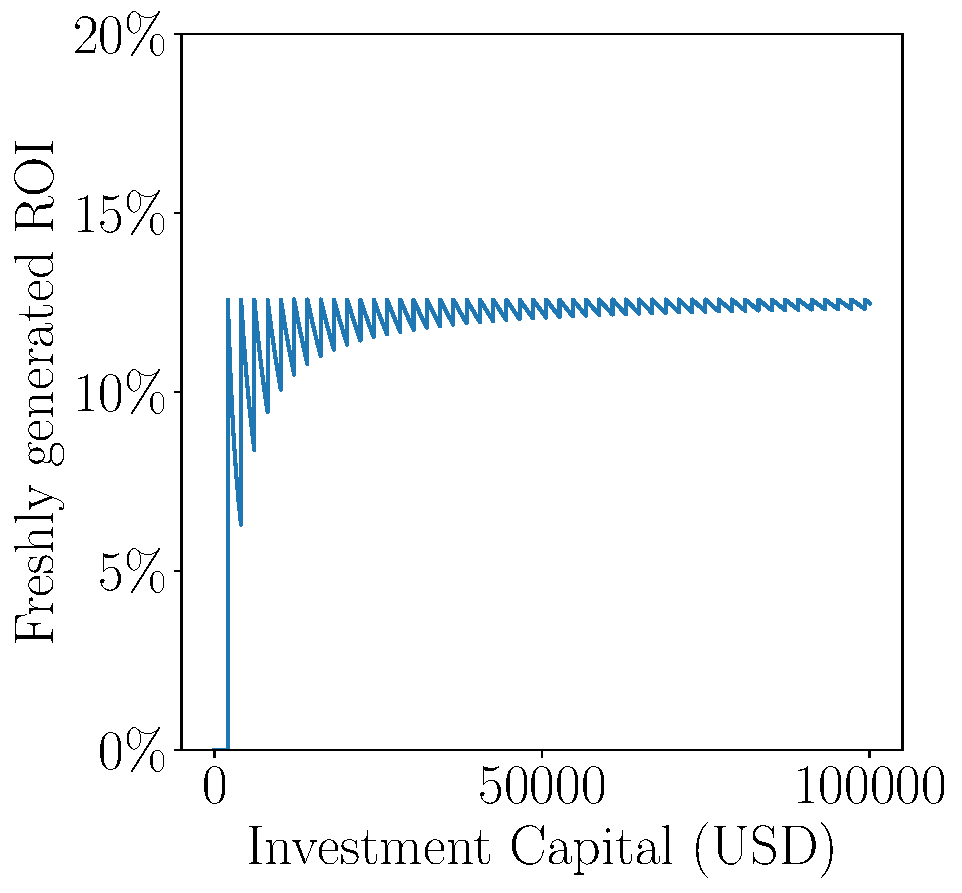
\includegraphics[width=0.75 \columnwidth,keepaspectratio]{figures/decred-stake.pdf}
    \label{fig:decred-stake}
\end{figure}

In the case of pure proof-of-stake, every coin has the same probability of being chosen, so that its owner is eligible to create a block. Specifically, consider the case of a cryptocurrency with $N$ coins in circulation. Whenever a block needs to be created, a coin is chosen, therefore each coin may be chosen with $1 \over N$ probability. Then the address which owns the chosen coin, in other words the stakeholder which controls this coin, is eligible to generate a block and receive the rewards associated with this operation. In our experiments, we assume that every block is associated with a constant reward which pertains to newly minted coins. Furthermore, since computational power does not affect the rate of block production, it is reasonable to assume that both the electricity and the hardware equipment's price is constant, such that all users can participate using a cheap machine.

Figure~\ref{fig:pure-pos-stake} depicts the simulation of a pure proof-of-stake system. In this case, the users pay a set fee which represents the hardware and electricity cost, whereas the rest of the capital is used to buy coins. It is clear that this system converges much faster than both proof-of-work and the hybrid case above.

\begin{figure}[H]
    \caption{The egalitarianism of \emph{staking} in a pure proof-of-stake cryptocurrency.}
    \centering
    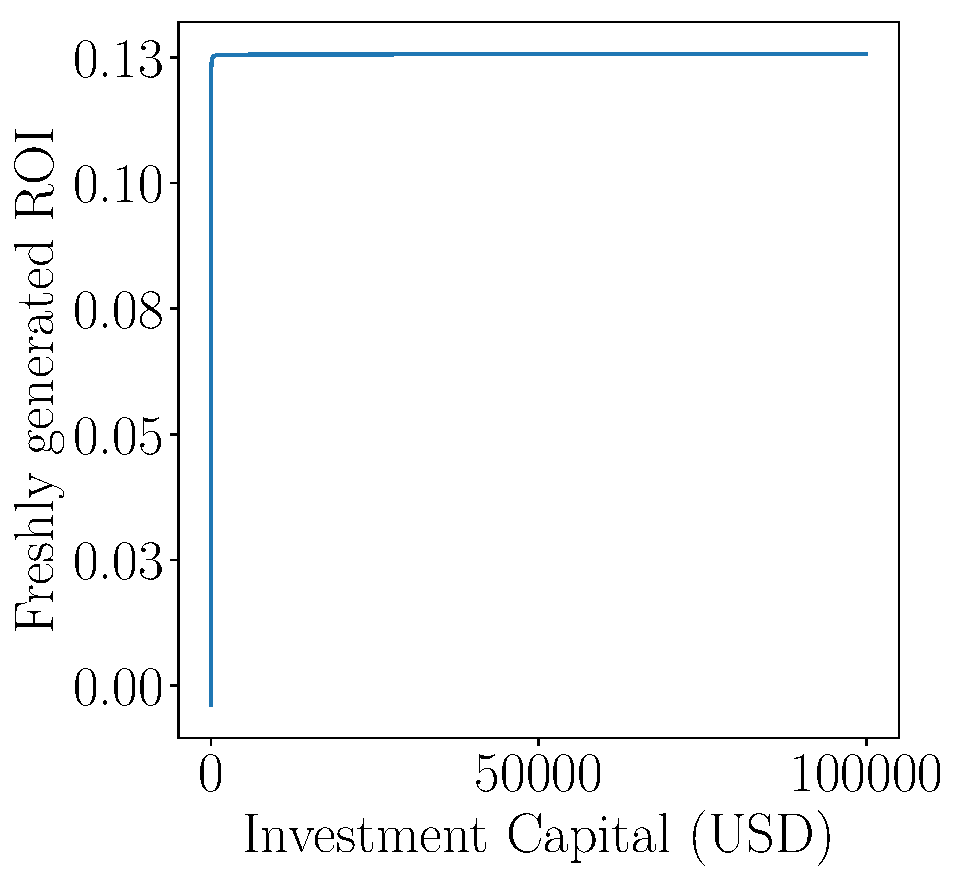
\includegraphics[width=0.75 \columnwidth,keepaspectratio]{figures/pure-pos.pdf}
    \label{fig:pure-pos-stake}
\end{figure}

\dionyziz{Add Ouroboros figure and discussion}

Our findings are summarized in Table~\ref{tbl:egalitarianism}. We find that
Bitcoin is the least egalitarian, followed by Ethereum, Litecoin, and Monero.
The latter two are the most egalitarian due to their use of scrypt and
Cryptonight respectively. Decred is a hybrid coin which can both be staked and
mined. Mining with Decred has egalitarianism which stands between Ethereum and
Litecoin. The most egalitarian coins involve staking. Decred staking, due to its
quantized ticket pricing, is only approximately egalitarian. Pure proof-of-stake, which
allows continuous staking, is perfectly egalitarian.

\dionyziz{Spelling of ``cryptonight''?}
\dionyziz{Carefully reread and revise findings of above paragraph}

\begin{table}
  \centering
  \begin{tabular}{|c|c|c|c|c|c|c|c|}
    \hline
    & Bitcoin & Ethereum & Litecoin & Monero & \multicolumn{2}{c|}{Decred} & Ouroboros\\
    \hline
    \textbf{Proof-of-work} &
    $\times$ & $\times$ & $\times$ & $\times$ & $\times$ & & \\
    \hline
    \textbf{Proof-of-stake} &
    & & & & & $\times$ & $\times$ \\
    \hline
    \textbf{Egalitarianism} &
    ? & ? & ? & ? & ? & ? & ? \\
    \hline
  \end{tabular}
  \caption{The egalitarianism of the various cryptocurrencies we studied.}
  \label{tbl:egalitarianism}
\end{table}

\dionyziz{Fill in numbers in above table}
